\textcolor{BrickRed}{\bf NOTA:}  Los ejercicios se encuentran repartidos en los archivos:
\begin{itemize}
	\item \textcolor{mediumblue}{ejercicio1.py}
	\item \textcolor{mediumblue}{ejercicio2.py}
	\item \textcolor{mediumblue}{ejercicio3.py}
	\item \textcolor{mediumblue}{ejercicio4.py}
\end{itemize}

% -----------------------------------------------------------------------------------------
\vspace{5mm}
{\color{lightgray} \hrule}
\begin{enumerate}
	\item Implementar el algoritmo de Gram-Schmidt modificado 8.1 del Trefethen (p. 58) para generar la descomposición QR.
\end{enumerate}
En el archivo \textcolor{mediumblue}{ejercicio1.py} se implementa el algoritmo de Gram-Schmidt modificado para calcular la factorización $QR$ de una matriz $A$ de $m\times n$ en la función \textit{MODIFIED\_GRAM\_SCHMIDT()}.

Acepta como argumentos a la matriz $A$ a factorizar y un booleano que indica si se sobreescribe la matriz $A$ (\textit{defatul = False}). Como salidas tiene a las matrices $Q$ y $R$ tales que $A = QR$ con $Q$ es una matriz ortogonal de tamaño $m\times n$ y $R$ es una matriz triangular superior de tamaño $n \times n$. Además, se incluye un par de ejemplos de uso de la función.

% -----------------------------------------------------------------------------------------
\vspace{5mm}
{\color{lightgray} \hrule}
\begin{enumerate} \setcounter{enumi}{1}
	\item Implementar el algoritmo que calcula el estimador de mínimos cuadrados en una regresión usando la descomposición QR.
\end{enumerate}

Dada una regresión lineal:
\begin{equation}
	y = X\beta+\epsilon
\end{equation}
donde $y$ es el vector de valores observados, $X$ es la matriz de diseño (de tamaño $m\times n$), $\beta$ es el vector de coeficientes de regresión y $\epsilon$ es el vector de errores. El objetivo es estimar $\beta$ que minimiza la función de pérdida de mínimos cuadrados, que es:
\begin{equation}
	\min_{\beta} \left\| y-X\beta \right\|^2.
\end{equation}
Con esto, se usa la descomposición $QR$ de la matriz $X$, donde $X = QR$, siendo:
\begin{itemize}
	\item $Q$ es una matriz ortogonal de tamaño $m\times n$.
	\item $R$ es una matriz triangular superior de tamaño $n \times n$.
\end{itemize}
$\implies y = QR\beta + \epsilon$ y como $ Q^{T}Q = I_{m\times m}\implies Q^{T}y = Q^{T}QR\beta = R\beta$ y se obtiene que
\begin{equation} \label{eq:sistema}
	R\beta = Q^{T}y.
\end{equation}
Como $R$ es triangular superior, podemos usar {\it backward substitution} de la Tarea 1. En el archivo \textcolor{mediumblue}{ejercicio2.py} se usa la función \textit{MODIFIED\_GRAM\_SCHMIDT()} del ejercicio 1 para crear la función \textit{LEAST\_SQUARES\_QR()}, la cual calcula la factorización $QR$ de una matriz $X$ para después resolver el sistema \eqref{eq:sistema} con ayuda de {\it backward substitution}.

% -----------------------------------------------------------------------------------------
\vspace{6mm}
{\color{lightgray} \hrule}
\begin{enumerate} \setcounter{enumi}{2}
	\item Generar $\mathbf{Y}$ compuesto de $y_i=\sin{\left(x_i\right)}+\epsilon_i$ donde $\epsilon_i \sim N(0, \sigma)$ con $\sigma=0.11$ para $x_i=\frac{4 \pi i}{n}$ para $i=1, \ldots, n$. Hacer un ajuste de mínimos cuadrados a $\mathbf{Y}$, con descomposición $Q R$, ajustando un polinomio de grado $p-1$.
	\begin{itemize}
		\item Considerar los 12 casos: $p=2,4,6,100$ y $n=100,1000,10000$.
		\item Graficar el ajuste en cada caso.
		\item Medir tiempo de ejecución de su algoritmo, comparar con descomposición $Q R$ de scipy y graficar los resultados.
	\end{itemize}
\end{enumerate}

Se tiene la expresión
\begin{equation} \label{eq:4}
	y_i = \sin{\left(x_i\right)} + \epsilon_i
\end{equation}
con $\epsilon_i \sim N(0, \sigma)$, $\sigma=0.11$ y $x_i=\frac{4 \pi i}{n}$ para $i=1, \ldots, n$. Se requiere ajustar un polinomio de grado $p-1$ a estos datos, es decir, se busca una relación del tipo:
\begin{equation} \label{eq:5}
	y_{i} \approx \beta_{0} + \beta_{1} x_i + \beta_{2} x_i^2 + \cdots + \beta_{p-1} x_i^{p-1}.
\end{equation}
para $i=1, \ldots, n$. Se puede escribir la ecuación anterior de forma matricial:
\begin{equation} \label{eq:6}
	\mathbf{Y} = \mathbf{X} \beta
\end{equation}
con
\begin{equation} \label{eq:7}
\mathbf{Y} = 
\begin{pmatrix}
	y_1 \\
	y_2 \\
	\vdots \\
	y_n
\end{pmatrix},\quad
\mathbf{X} = 
\begin{pmatrix}
	x_{1}^{p-1} & x_{1}^{p-2} & \cdots & x_{1} & 1 \\
	x_{2}^{p-1} & x_{2}^{p-2} & \cdots & x_{2} & 1 \\
	\vdots & \vdots & \ddots & \vdots & \vdots \\
	x_{n}^{p-1} & x_{n}^{p-2} & \cdots & x_{n} & 1
\end{pmatrix},\quad
\beta = 
\begin{pmatrix}
	\beta_{p-1} \\
	\beta_{p-2} \\
	\vdots \\
	\beta_{0}
\end{pmatrix}
\end{equation} 
Dado esto, se puede usar a la matriz $\mathbf{X}$ como matriz de diseño para resolver el problema:
\begin{equation} \label{eq:8}
	\min_{\beta} \left\| \mathbf{Y} - \mathbf{X}\beta \right\|^2.
\end{equation}
Tomando la factorización $QR$ de $\mathbf{X}$ ($\mathbf{X} = \mathbf{QR}$), se puede resolver el sistema:
\begin{equation} \label{eq:9}
	\mathbf{R}\beta = \mathbf{Q}^{T}\mathbf{Y}
\end{equation}
con ayuda de {\it backward substitution} (ya que $\mathbf{R}$ es triangular superior).

En el archivo \textcolor{mediumblue}{ejercicio3.py} se implementa la función \textit{AJUSTE\_QR()} que da la generación de $\mathbf{Y}$ como se muestra en \eqref{eq:4}. Con ayuda de la función \textit{vander()} de la librería \textit{numpy}, se crea la matriz $\mathbf{X}$ dada en \eqref{eq:7} y se resuelve el sistema \eqref{eq:9} para $\beta$ con ayuda de la función \textit{BACKWARD\_SUBST()} de la Tarea 1 y con la factorización obtenida por \textit{MODIFIED\_GRAM\_SCHMIDT()}. Posteriormente, se calcula la estimación $\hat{\mathbf{Y}} = \mathbf{X} \beta$ y tiene como salidas: $x_i, y_i, \beta$ y $\hat{y}_i$.

Se consideran los casos para $p=2,4,6,100$ y para $n=100, 1000, 10000$. No se imprime ninguna de las características $x_i, y_i, \beta, \hat{y}_i$ para no abrumar el espacio de código. Se generó cada una de las gráficas de los ajustes y se imprimen a continuación en una sola figura. Es importante destacar que en este caso, se usó la función \textit{MODIFIED\_GRAM\_SCHMIDT()} para la factorización $QR$ involucrada.
\begin{figure}[h!]
	\centering
	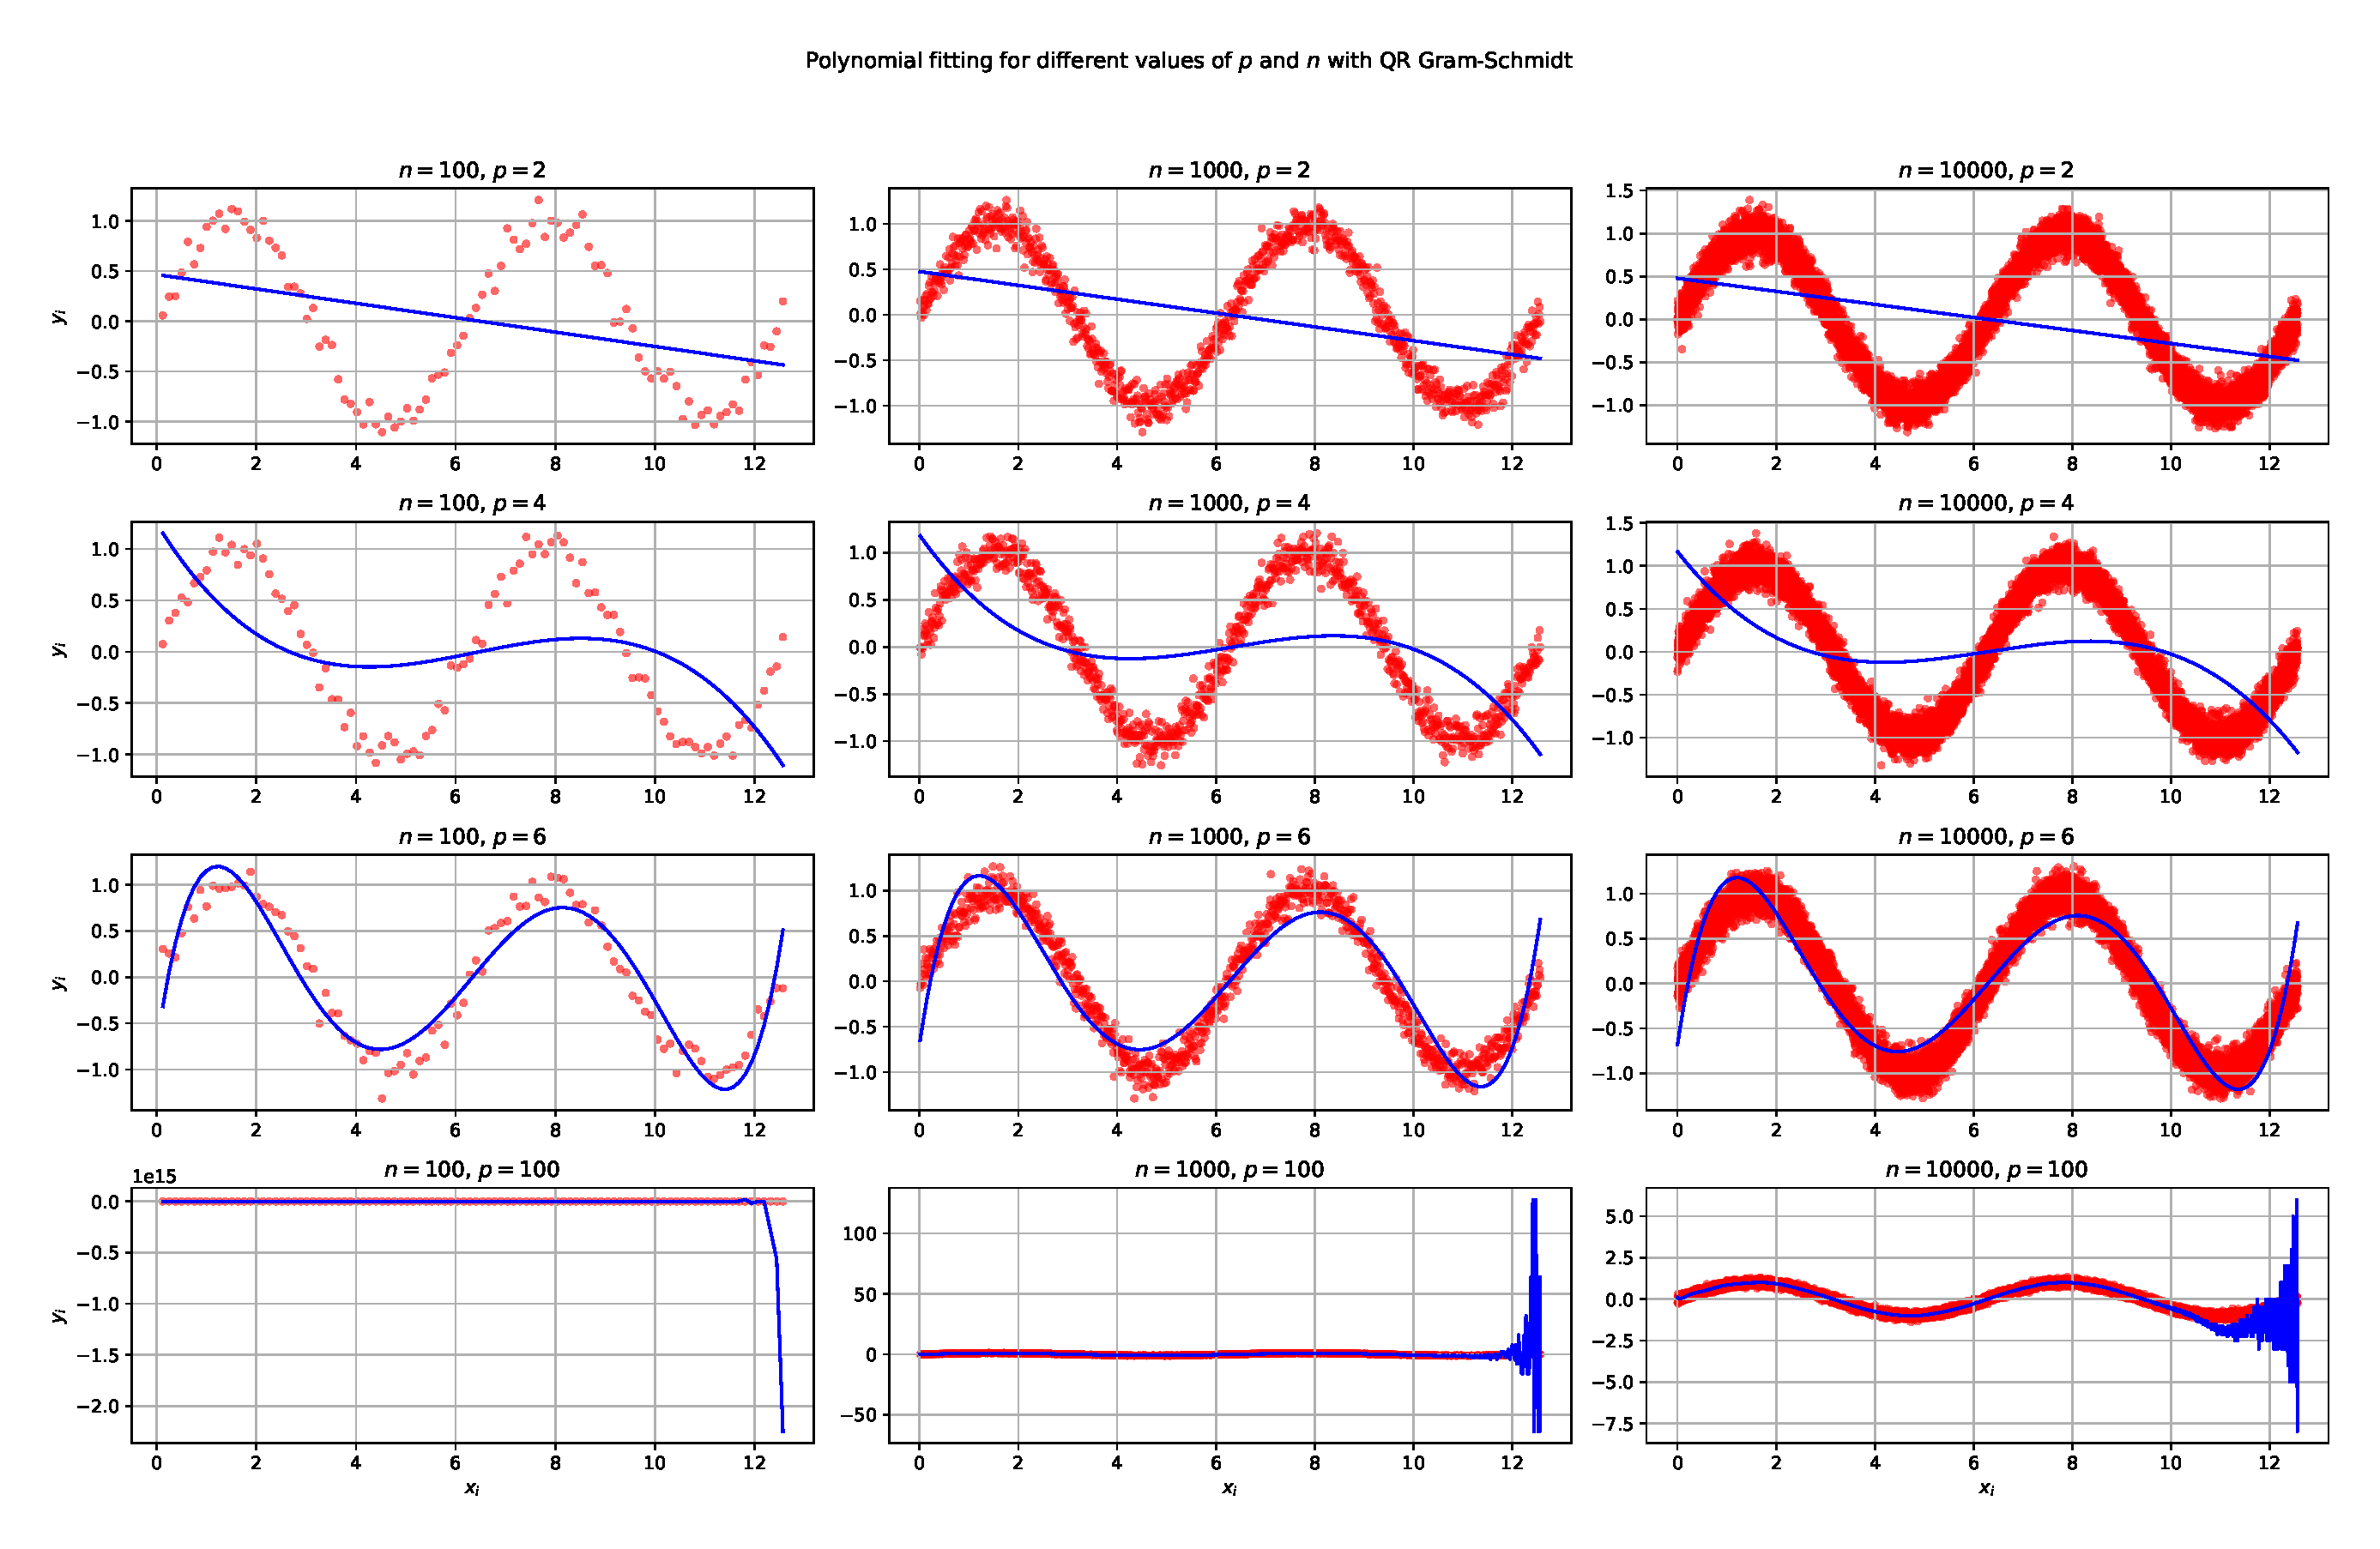
\includegraphics[width=\textwidth]{IMAGENES/gram_schmidt.pdf}
\end{figure}

\vspace{2.5cm}
Lo mismo se repitió haciendo uso de la descomposición $QR$ de scipy, generando los siguientes resultados gráficos:
\begin{figure}[h!]
	\centering
	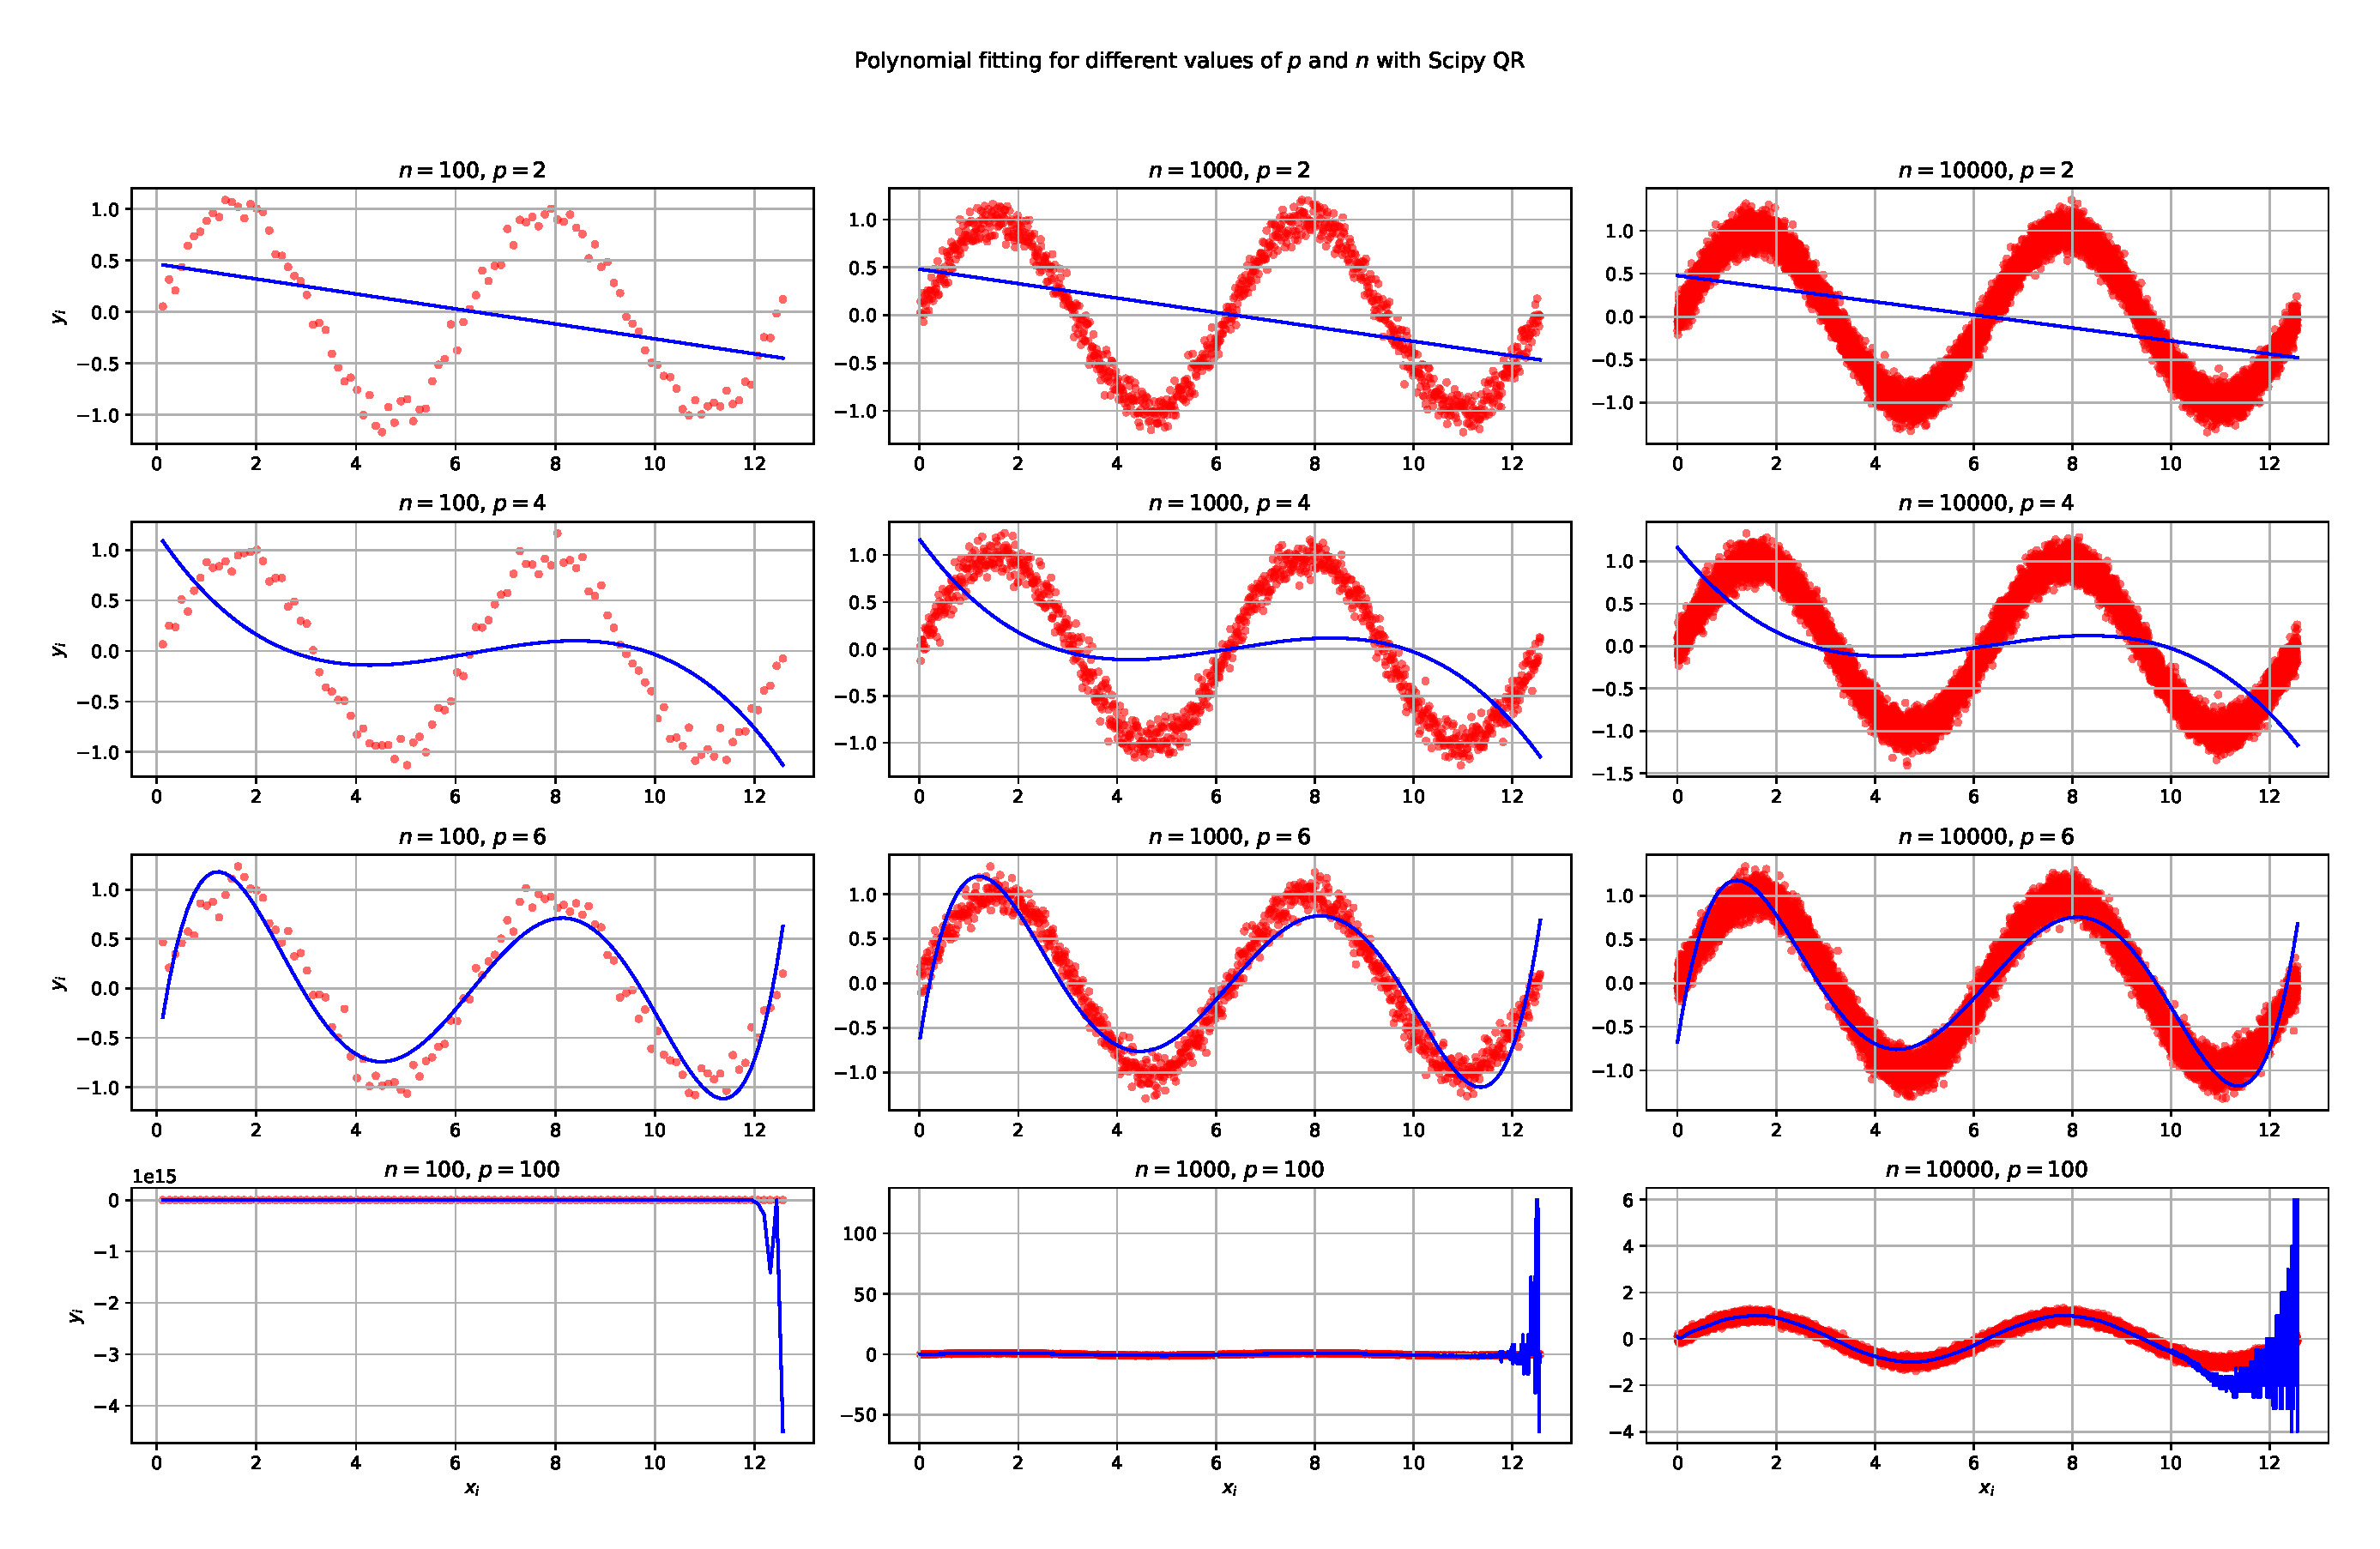
\includegraphics[width=\textwidth]{IMAGENES/scipy.pdf}
\end{figure}

Además, se obtuvo la siguiente tabla al momento de comparar los tiempos de ejecución en segundos de ambos métodos:

\begin{table}[h!]
	\centering
	\begin{tabular}{|c|c|c|c|}
		\hline
		          & QR de Gram-Schmidt  & QR de Scipy  & Scipy - Gram-Schmidt  \\ \hline
		$p=2$ y $n=100$  & 7.5667e-05  & 0.0001  & 4.4916e-05  \\ \hline
		$p=2$ y $n=1000$  & 7.6832e-05  & 7.6791e-05 & -4.1999e-08  \\ \hline
		$p=2$ y $n=10000$  & 0.0216  & 0.0003  & -2.1351e-02  \\ \hline
		$p=4$ y $n=100$ & 6.5249e-05  & 4.2833e-05  & -2.2417e-05  \\ \hline
		$p=4$ y $n=1000$  & 0.0001  & 7.1166e-05  & -3.7043e-05  \\ \hline
		$p=4$ y $n=10000$  & 0.0228  & 0.0004  & -2.2407e-02  \\ \hline
		$p=6$ y $n=100$  & 7.7917e-05  & 4.2042e-05  & -3.5875e-05  \\ \hline
		$p=6$ y $n=1000$  & 0.0001  & 8.6792e-05  & -6.3749e-05  \\ \hline
		$p=6$ y $n=10000$  & 0.0199 & 0.0018 & -1.8163e-02 \\ \hline
		$p=100$ y $n=100$  & 0.0129 & 0.0958 & 8.2915e-02 \\ \hline
		$p=100$ y $n=1000$  & 0.0244 & 0.2927 & 2.6833e-01 \\ \hline
		$p=100$ y $n=10000$  & 0.2044 & 0.3147 & 1.1026e-01 \\ \hline
	\end{tabular}
	\caption{Comparación de tiempos de ejecución en segundos.}
\end{table}

\textbf{NOTA:} Los resultados pueden variar en cada ejecución del archivo \textcolor{mediumblue}{ejercicio3.py} ya que depende de la situación de la memoria del dispositivo actual. El comportamiento en cada uno de ellos es bastante similar.

Se exhiben los tiempos de ejecución de ambos algoritmos para cada caso y en la tercera columna se da la diferencia de estos tiempos. Se puede notar que casi todas estas diferencias son negativas, por lo que concluye que la implementación de la factorización $QR$ de Scipy es más rápida que la implementada en el ejercicio 1.

% -----------------------------------------------------------------------------------------
\vspace{5mm}
{\color{lightgray} \hrule}
\begin{enumerate} \setcounter{enumi}{3}
	\item Hacer $p=0.1 n$, o sea, diez veces más observaciones que coeficientes en la regresión, ¿Cual es la $n$ máxima que puede manejar su computadora?
\end{enumerate}

En el archivo \textcolor{mediumblue}{ejercicio4.py}, se tiene la implementación y graficación para diversos valores de $n$ y $p=0.1n$. Se intentó para valores muy grandes de $n$ (en particular, el entero más grande reconocible por la computada es $10^{4300}$), sin embargo, lo que ''desaparecía'' era el ajuste polinomial bastante antes. Es decir, para valores grandes de $n$, la generación de puntos se realizaba después de un largo tiempo, pero el polinomio de grado $p$ nunca se generaba debido a indeterminaciones en la ejecución de la función \textit{MODIFIED\_GRAM\_SCHMIDT()}.

Debido a esto, fue necesario encontrar el $n$ tal que $p=0.1n$ no generara problemas a la hora de hacer el polinomio de grado $p$. Se llegó a la conclusión que para valores de $p$ mayores a $281$, $i.e., n>2819$ resultaba imposible hacer el ajuste:

\begin{figure}[h]
	\centering
	\begin{minipage}{0.495\textwidth}
		\centering
		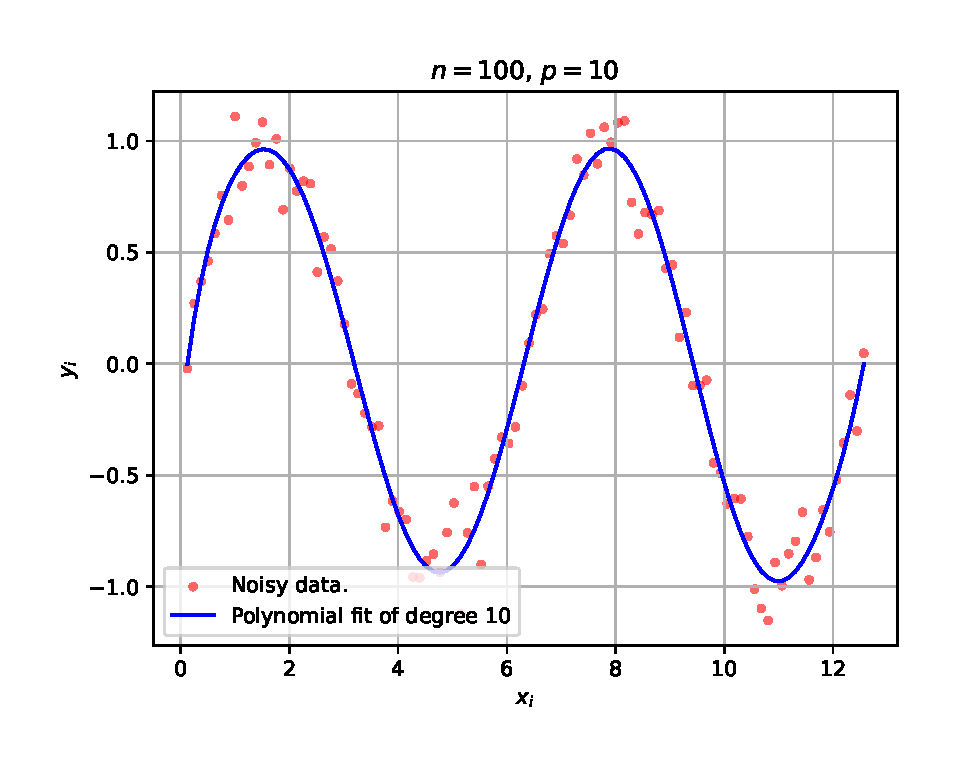
\includegraphics[width=\textwidth]{IMAGENES/n_100_p_10.pdf}
		\caption{$n=100, p=10$.}
	\end{minipage}
	\hfill
	\begin{minipage}{0.495\textwidth}
		\centering
		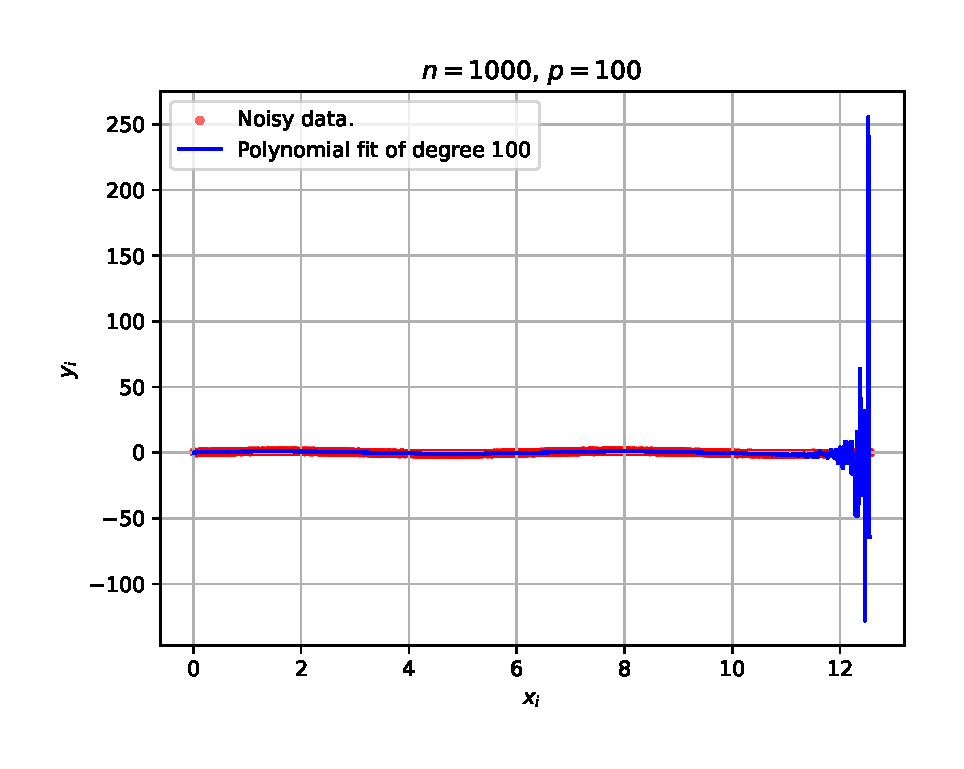
\includegraphics[width=\textwidth]{IMAGENES/n_1000_p_100.pdf}
		\caption{$n=1000, p=100$.}
	\end{minipage}
\end{figure}

\begin{figure}[h!]
	\centering
	\begin{minipage}{0.495\textwidth}
		\centering
		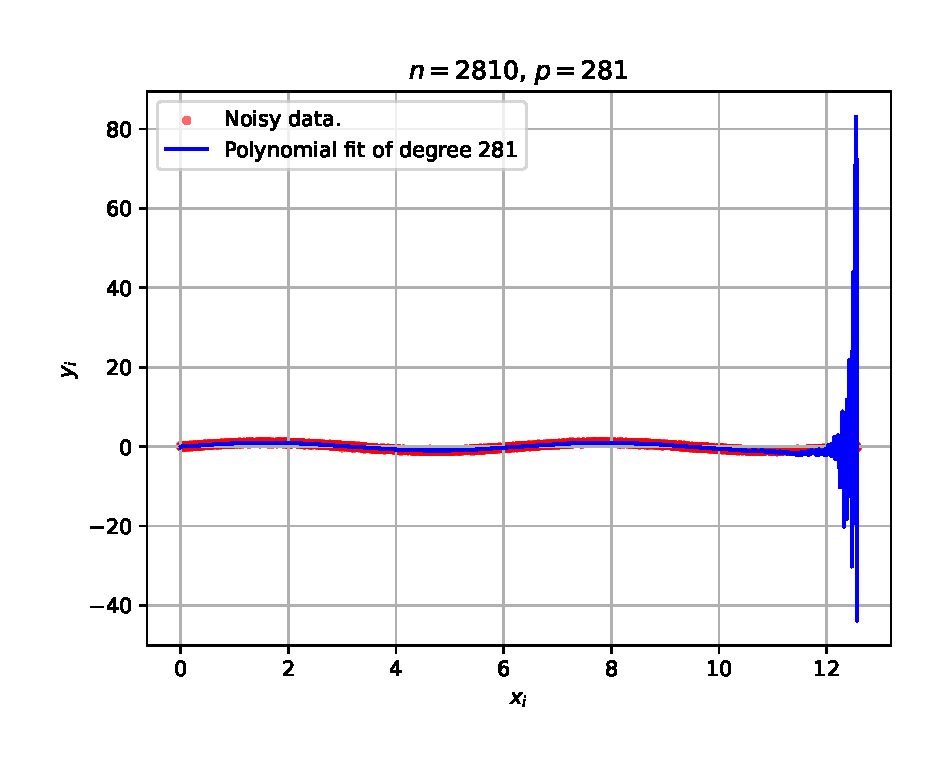
\includegraphics[width=\textwidth]{IMAGENES/n_2810_p_281.pdf}
		\caption{$n=2810, p=281$.}
	\end{minipage}
	\hfill
	\begin{minipage}{0.495\textwidth}
		\centering
		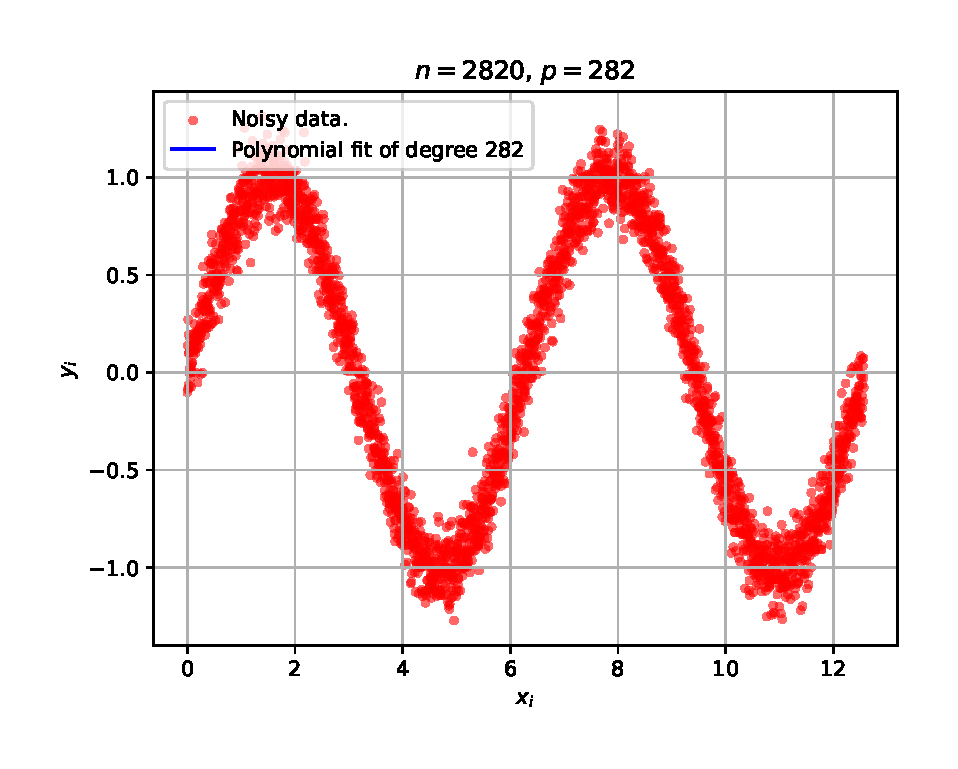
\includegraphics[width=\textwidth]{IMAGENES/n_2820_p_282.pdf}
		\caption{$n=2820, p=282$.}
	\end{minipage}
\end{figure}

Además, se hicieron simulaciones para $n$ todavía más grande, sin embargo, el resultado era el mismo: los datos con ruido se generan, pero el polinomio no:

\begin{figure}[h!]
	\centering
	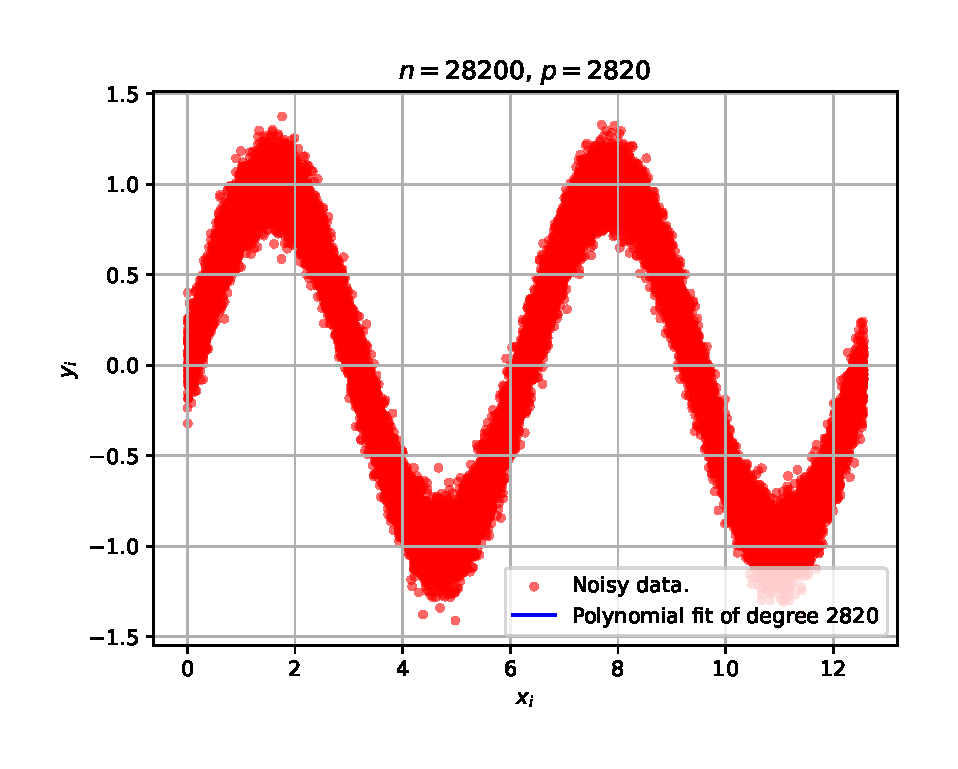
\includegraphics[width=\textwidth]{IMAGENES/n_28200_p_2820.pdf}
\end{figure}









